\chapter{Test}\label{ch:test}
The primary test purpose is to reveal the presence of faults in a system. The main idea behind testing consists in applying test data to inputs of the IC, design, wafer, dice, or any other system called Unit Under Test (UUT) and collecting data from its outputs. The test data applied to the inputs is called the test vector or test stimuli and the data collected from the outputs - the response of the UUT. The term test pattern is used to describe the test vectors together with expected correct responses. A test set relates to a series of test patterns. After applying test vectors and capturing the responses, they are compared with a fault free response stored in the test pattern. If they differ in any position or value, fault is uncovered. The \autoref{fig:test} shows the typical test environment

\begin{figure}[H]
\centering
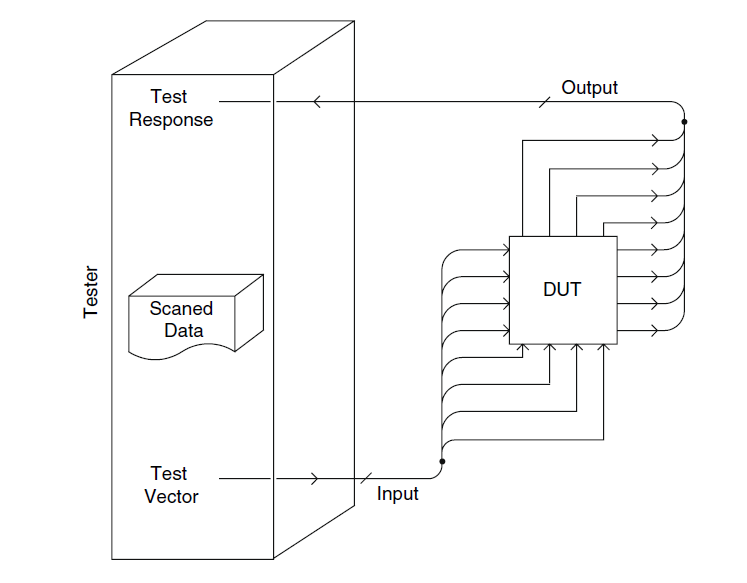
\includegraphics[width=0.65\textwidth]{figures/test.png}
\caption{The tester principle~\cite{book:Navabi}}
\label{fig:test}
\end{figure}


\section{Fault models}

While it is possible to prove the presence of faults in the design, there is no method proving their absence. The amount of different faults and their variety is countless, hence there are means needed to model how those faults affect the system. The fault itself is not visible to the tester itself (except from visual tests) and has to be stimulated to manifest, and in best case, propagate to the UUT outputs. Many different faults can have the same effect, so investigating the effects of faults may bring better results. The fault effects are called failure modes and they have to be modeled in order to conduct tests. Such fault models serve the purpose of altering the data flow, in the similar way, as the real faults would. It allows to develop test vectors to stimulate and propagate the real faults effects. There are two groups of fault models. The ones that describe faults affecting the logical operations and ones describing the defects in parameters. The most common logical fault models are:
\begin{itemize}
    \item Stuck-At-Fault consists in an assumption that a node in the design has a permanent value and doesn't respond to the logical transitions forced on it. The node can be Stuck-at-0 (SA0) or Stuck-at-1 (SA1)
    \item Bridging fault assumes that two nodes interact with each other unintentionally producing either a Wired-AND effect with 0-dominant connection or Wired-OR effect being 1 dominant.
    \item Delay fault may be considered as a parametric fault rather than a logic fault. The net delay fault occurs when a signal needs more time, to cover certain logical path, then assumed. The transmission delay faults describe the situtation when the fault is caused by fall and rise times of clock signal driving the logical gate, when the signal doesn't make it from the input to the output during one clock cycle. The result may be the previous value processed by consecutive gates or delayed value stored in a memory cell.
    \item Memory fault (logical faults considered)
    \item Single Event Transient (SET) describes a glitch in combinational logic that travels trough design.
    \item Single Event Upset (SEU) describes the situation when the incorrect voltage level caused by SET gets stored in the memory or the memory state changes. Can affect more memory cells at once.
    \item Single Event Latchup (SEL) - a highly loaded particle makes a locked transistor conduct leading to short in CMOS logic. Requires a power reset and may lead to a hard fault, because of a very high temperature~\cite{report:altera}.
\end{itemize}
The parametric faults are modeled through:
\begin{itemize}
    \item Bridging fault assumes resistive unintentional connection between two nodes
    \item Memory fault (non-logical faults considered)
    \item Open-circuit fault in interconnect metal
    \item Stuck-open and stuck-short faults in transistors
    \item $I_{DDQ}$ Fault - measuring the current by power supply during static operation of the design (while there is no switching activity)
\end{itemize}
All mentioned models represent failure modes in digital hardware logic, even the analog or mixed signal tests consider only digital circuits. Most operations however take less time and energy when moved from digital domain to analog one. Additionally every radio related circuit does some, or even majority of operations in analog domain and mixed-signal domain. In modern communication systems, with SoC technology, there is a rapid growth in analog and mixed circuitry that is also vulnerable to faults. The number of such faults is again countless and some sort of abstraction is required. The continuous characteristic of analog systems allows only for two fault models:
\begin{itemize}
    \item Catastrophic failures - the system is not functional at all
    \item Unacceptable performance - the service is still provided but some of the functionality lies outside of the acceptable range of the specification
\end{itemize}
The border line between those two is obviously very subjective and bases on the definition of system correct functionality.~\cite{book:Kabisatpathy}.
\section{Test Types}
Testing can be done in following ways:
\begin{itemize}
    \item External testing is when the design is tested by some external circuit from the tested design perspective. The internal testing assumes that all needed components are integrated in the circuit, like in case of the Built In Self Test described later.
    \item Online testing doesn't disturb hardwares normal operation, while an offline test requires the system to stop working for the test to be carried out.
    \item Concurrent testing is online testing that is carried out with normal data sets while normal system function.
    \item At-speed testing is conducted at normal speed of the design instead of lowered frequency, that needs to be specially generated for test purpose. To realize at-speed testing often a second, shifted frequency is required.
    \item Diagnostic test is carried out to find a cause of a failure
\end{itemize}

\section{Design For Testability (DfT)}
If the test vectors can only be applied to the unit inputs and responses sampled only from the outputs, many problems occur. While testing, the combinational fan-outs and reconvergences become problems. To stimulate faults laying deep inside the combinational logic structure, the test designer has to come up with such a vector, that will force a certain state in the logic and let this state propagate to one of the design outputs. Testing sequential logic in this way would be nearly impossible because of the complexity of creating and testing all possible states of such system. Therefore the testability has to be supported by system designers to allow test access to those parts of the design, that are difficult to test using only primary inputs and outputs. Incorporating the testability methods in the design work flow is called the Design For Testability and is a standard approach during the development of todays complex electronic systems. The designers have many options in making their designs easier to test, therefore maximizing the test coverage. Ease of test is meant both by reduced complexity of test and by easier physical access to the system. The means for testability are listed below.
\subsection{System Partitioning}
To increase testability the untestable complex systems have to be split into smaller testable units. If one wanted to test a 64-bits counter and compare each time against correct data, the test could take years. Splitting the counter into 4 16-bit counters reduces the test time to nearly half of a second. The tester has to deal with just 4 16 bit counters, that can be tested in parallel which would be impossible with one big counter.

Another example of partitioning is based on the knowledge how the sequential logic is built. Synchronous sequential systems can be represented as combinational logic with delayed feedback. The delay is implemented as flip-flops which separate the actual state of the system from its next state. The whole system can be therefore understood as the Meely state machine and is shown in the \autoref{fig:Meely}. Most of the logic gates reside in the combinational part, so the test procedure should focus on this part. Gaining access to present state inputs, together with manipulating the primary inputs, would allow the tester to determine an exact state of the system and test it.

\begin{figure}[H]
\centering
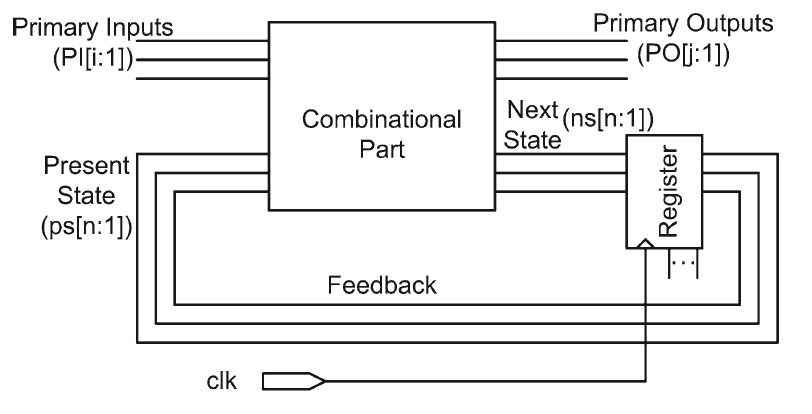
\includegraphics[width=0.65\textwidth]{figures/Meely.PNG}
\caption{Representation of a sequential system as the Meely state machine \cite{book:Navabi}}
\label{fig:Meely}
\end{figure}

\subsection{Scan test}
The "divide and conquer" approach allows other widely used methods to be implemented. The most common and supported method is a scan test. It exploits the method of unfolding the sequential logic into combinational part and memory feedback part. The flip-flops containing the present state of the system on their outputs and the next state of the system on their inputs are transformed into one big shift register. In normal mode the shift register is treated as parallel input parallel output register, with shifting option disabled. When the test takes place, the data is serially shifted through the shift register until all registers reach their determined state. The data is then shifted out for comparison. The shifting can be clocked with much higher frequency then the system is designed for, because until all registers are filled with data, the output of the combinational logic is irrelevant. The fast clocking can however lead to abnormal power consumption and heat emission and in result to systems premature deterioration. The test parameters have to be adjusted with care. The scan test is a crucial part of boundary scan technology, where scan path can be accessed as IO of the IC. The test pattern generation and response analysis is usually placed externally from the UUT and used only during the test procedure, for example during the post-manufacturing tests. The tools for pattern generation and response analysis are named Automatic Test Equipment (ATE) and can be dedicated to one chip or universally adaptable to test many different architectures. The configurable solution lowers the test costs and development time. Placing the test logic outside of the chip simplifies its design and lowers the complexity of the system.

\subsection{Buit-In-Self-Test (BIST)}
The test access to the IC is not only relevant during a post manufacture testing and should be possible not only with use of ATE. Many safety-critical or mission-critical applications require the unit to be able to conduct a local self tests autonomously and detect its own errors. The integration of test logic in the chip itself can also speed up the test process. The test equipment would only start the test routine and read the outcome. The Built-In-Self-Test consists of scan path, test pattern generator and output response analyzer integrated into the design. The test pattern generation is often conducted with the use of LFSR and its pseudo-random output. The patterns may also be stored in a ROM in a compressed form. The output response analyzer can compare either the whole input bit stream or just the signature of the response, in hope that they are different from the pre-calculated, fault-free signature. This approach may lead to undetected faults in cases of collisions in the signature generation algorithm.

\subsection{Analog and Mixed-Signal DfT}\label{sub:testa}
Together with the todays trend of integrating digital, analog and mixed-signal logic into one System-On-The-Chip (SoC), the external test of non-digital parts of the design is no longer sufficient. The mixed circuitry gets also widely implemented into safety- and mission-critical applications and requires appropriate DfT techniques.

The main drawback in adopting standard DfT techniques into an analog domain is the degradation of the signal quality, when any additional circuitry is being added to the signal paths. There is a mixed-signal test bus standard (IEEE Std 1149.4-1999) which provides a boundary scan capability, improving the controllability and observability of the design, but leaving the response analysis and wave generation to the ATE. Another problem is the not-ideal response of switches, which can distort the signal even when in normal mode.

There is no standardization of BIST techniques and most of the implementation tend to be ad-hoc. The on-chip analog test pattern generation has been proven to work with the use of Pulse Density Modulated signals, followed by low pass filters to create a wave of desired shape. The more "ones" following each other, the higher the amplitude of the output signal. The PDM signal is digitally generated and the response can be sampled back into the digital domain for comparison or evaluation. The sampling is possible thanks to the Delta-Sigma Modulator ($\Delta \Sigma M$), which recreates the digital bit stream with the density of ones proportional to the analog signal~\cite{book:Grout}.

The response analysis is another demanding task, usually done externally by ATE, together with sampling the output voltage and currents. With use of the Delta-Sigma Modulator or another ADCs, the analog signals can be evaluated as digital bit streams. The latest development in machine learning technologies proved to be successful in evaluation of many voltage levels coming from an RF chip and classifying them as faulty or fault-free~\cite{art:neural}.

In communication systems, the extra hardware cost and performance degradation could be omitted by usage of the existing converters for test purposes. The transceivers contain units, that given a digital bit stream convert it to the analog signal to be modulated with the carrier wave. If the output of such module would be connected to the input of corresponding unit in the receiver, responsible for recreation of digital information from analog signal returned by demodulator, then the analysis of this digital output signal, could reveal errors in one of the modules.